%%
%% Author: shoupu_wan
%% 11/18/18
%%

\chapter{Cascading Conditionals}\label{ch:conditional-cascade}

A sequence of three or more tightly coupled conditional statements as shown in
~\autoref{lst:simpleBranching} is probably familiar to reader.
Similar structures are not uncommon even in programing primer books.
Many times, it begins with an \code{if}-conditional, optionally followed by one or more
\code{else if} (or \code{elif}) blocks, and optionally ends with an \code{else} block.
For the sake of discussion in this book, we refer to such a train of conditional statements
collectively as `\emph{cascading conditional construct}';
sometimes we use `\emph{cascading conditional}', even simply `\emph{cascade}',
or shorthand \emph{CC}  interchangeably.

Occasionally when it is the last statement to be executed in a function
or a loop, cascading conditional may take the form of a sequence of \code{if} statements
in conjunction with \code{return}, \code{continue},
\code{break}, \code{exit}, \code{yield} and other branching statements (instead
of `\code{if..elif..elif..}').
Regardless of the form, the distinguishing characteristics of a cascading conditional are
the `tight coupling' and `sequential order' among the constituent conditional statements.
Below are some examples of cascading conditionals
\begin{clisting}[h]
    \begin{minipage}[t]{.4\textwidth}
        \lstinputlisting[label={lst:cascadeCondElif},
        caption={CC in \python}]
        {if-else/staircase_conditional.py}
    \end{minipage}\hfill
    \begin{minipage}[t]{.4\textwidth}
        \lstinputlisting[label={lst:cascadeCondReturn},
        caption={CC with keyword \code{return}}]
        {if-else/staircase_conditional_return.py}
    \end{minipage}
\end{clisting}


%with \code{return} statements in
%the block, or \code{break} and \code{continue} statements if used in a loop construct
%(conditional statement in loop will be discussed later in this chapter and in ~\autoref{ch:loops})

Cascading conditional is often used as a better alternative to nested conditionals
when facing multi-branch switching.
As ~\autoref{lst:nestedBranching} shows at the beginning of this chapter,
nested conditionals may be used for multi-branch switching.
However as the number of branches increases, nesting level as well as indentation level goes deeper.
The logic becomes unwieldy before long.
In contrast, cascading conditional offers compact logic and simple layout,
as shown in ~\autoref{lst:simpleBranching}.


Though cascading conditionals are ubiquitous in programming,
more often than not, developers' first experience with it begins with a `haphazard stumbling upon',
because seldom any systematic discussion exists to clarify the best practices surrounding it.
Used in conjunction with loops or recursive functions,
cascading conditional is an important programming construct for algorithmic implementations,
though it was not formally regarded as one in popular programming references.
For practical reasons, I am going to explain the use patterns of cascading conditional in this
section.
But rest assured that you will see its applications throughout this book---in
~\fullref{ch:loops}, ~\fullref{ch:recursion}, ~\fullref{lst:silhouette-skyline}, just to name a few.


First, let's begin with characterizing cascading conditionals.


\section{Cumulative Tests in Cascading Conditional}\label{sec:cumulativetests}

The tests in cascading conditional has cumulative effect.
To understand what this is and why, let us see how cascading conditional is executed.
Execution of a cascading conditional is analogous to stepping up a cascade.
The control successively evaluates the conditional expression and builds up the cases---the
leading conditional expression is checked and if evaluated to \code{true}, then the
first conditional block is executed and the rest is skipped;
otherwise, the next conditional expression is evaluated \ldots and so on.


As can be seen, the program acquires one assertion through each test in a cascading
conditional, as if collecting a stamp in the course of a scavenger hunt.
This is the `cumulative effect' of tests in cascading conditional as
illustrated in ~\autoref{lst:cumulative-tests-cascade}.


\begin{clisting}[tbh]
    \centering
    \lstinputlisting[caption={Expanded conditionals equivalent to
    ~\autoref{lst:cascadeCondElif} (in \java)},
    label={lst:cumulative-tests-expanded-equivalent}]
    {if-else/case_stack_taken_apart.java}
    %    \caption*{Cumulative effect of tests in a cascading conditional construct.
    %    Note the strict ordering on the left and loose grouping on the right.}
\end{clisting}

One of the key advantage of using cascading conditional is to reduce the number of cases one has
to check.
This reduction in number of tests would be made clear if one expands the cascading conditional
into non-cascading conditionals.
For example, in ~\autoref{lst:cumulative-tests-cascade} the number of tests checked is $3$
whereas in its expanded non-cascading equivalent in
~\autoref{lst:cumulative-tests-expanded-equivalent} it is $9$.
Cumulative effect saves us from retesting what's already tested and thus is one of the key factors
contributing to this test reduction.


The cumulative effect of cascading conditionals put a strict ordering among
its conditional statements.
At the same time, because of the cumulative effect, one has to commit more information in memory
at development time.
It is more challenging to keep one's mind synchronized with one's code
when programming cascading conditionals.
From this point of view, working out an expanded non-cascading equivalent such as
~\autoref{lst:cumulative-tests-expanded-equivalent} will be a useful exercise
when debugging cascading conditional in ~\autoref{lst:cumulative-tests-cascade}.


\section{How to Arrange Conditionals in Cascading Construct}
\label{sec:orderingstaircaseconditional}

Therefore arranging the conditionals in a cascading conditional construct is the key
from every point of view.
Apparently it will take considerable deliberation in order to produce correct, optimal and succinct
cascading conditional.
It is strongly recommended that reader use due diligence to screen and arrange tests in a cascade
conditional construct.
%This exerts a demanding requirement on empirical development expertise when it comes to design of
%cascading conditional.


The problem solving process goes as follows.
First, brainstorm on all the possible cases based on the project/problem requirement.
The key of this step is \emph{complete coverage} of all possibilities.
These cases may overlap with one another and which may or may not requires separate handling later.
Each problem has a unique set of conditions to be tested
which is essentially a multidimensional binary space partitioning problem\cite{NAYLOR90,NAYLOR93}.
As the cases are being tested, the solution space is also chopped in halves and
ruled out much like that of a binary search.
The BSP scheme for ~\autoref{lst:cascadeCondElif} is plotted in ~\autoref{fig:bsp}.

%These are usually the fundamental puzzle pieces which can be joined together to form larger parts.
%To visualize the idea, it is helpful to borrow concepts from binary space partitioning
%problem.
%On the other, classification of the problems is usually based on multiple conditional tests
%and partitions of them straddling across dimensions.
\begin{figure}[tb]
    \centering
    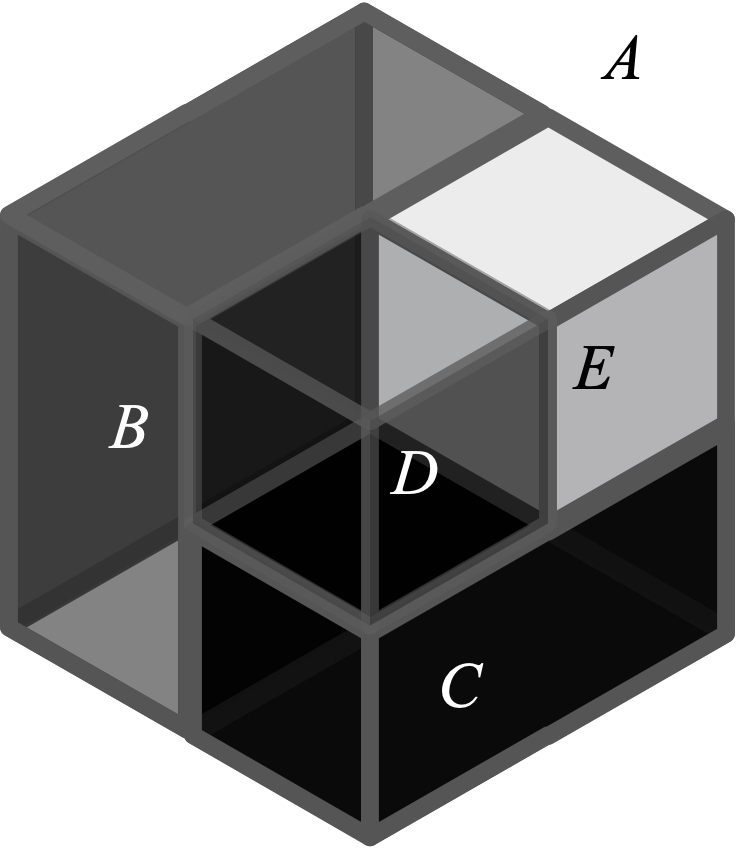
\includegraphics[width=.6\textwidth]{if-else/binary-space-partition.jpg}
    \caption{\label{fig:bsp}A sequence of tests performs binary space partitioning.
    \code{test1} partitions the whole space $A$ into two halves (labeled as $B$ is
    the `\code{true}' space);
    \code{test2} continues to partition the other half into two halves (labeled as $C$ is
    the `\code{true}' space);
    \code{test3} then partitions the remaining half into $D$ (`\code{true}')) and $E$
    (`\code{false}').}
\end{figure}


Secondly, examine the cases and attempt to eliminate or combine unnecessary cases.
The key success index for this step is \emph{non-overlapping, non-fragmenting} cases.
For example in programming for `binary search' based algorithms, one frequently faces a trichotomy
situation: \textit{less than},\textit{equals}, or \textit{greater than}.
Usually one does not need to test all three separately.
Instead, one only need to test two of the three---\textit{e.g.}  test for \code{less than} and
\code{greater than} and if both fail then it must be the third case.
Similarly in ~\autoref{lst:lca-skew-first}, one faces the quadchotomy: both keys
located on the left subtree, on the right subtree, key \code{a} on left subtree and key \code{b} on
right, or vice versa.
But I combined the cases such that only three cases are necessary: that both keys are located on
the left, on the right, or that they straddle over the root node.


Thirdly, with the consolidated distinct cases in hand, try to discover clues
that suggest certain order for them.
The most prominent clue is the dependency graph--some test is depended by others
(like nullity check).
This would form a directed acyclic graph among the tests.
In my own experience, I rarely needed to draw a DAG for this---just a simple rule of thumb worked.
But for complicated situations it may be beneficial to do so.
So topological ordering among the tests will put a strong constraint on how we can arrange the
tests within the cascading conditional.


Another clue comes from trichotomy or quadchotomy logic as we considered in the second step.
Using the example in ~\autoref{lst:lca-skew-first} again, I first test if both keys are
located on the left or right.
If neither, then it must be the straddling case.
I did not start with the straddling case because that test is in the `middle of the thick'.
If I do it first, I still have to chase down the left and back down the right.
It is a total waste.
Generally speaking, we should start with more `exposed', more accessible `edge cases' or `corner
cases' and gradually working our way into the thick of the puzzle.


More clues may be based on convenience or convention (following left \textit{v.s.}
right branch first), performance considerations (\textit{e.g.}, postpone costly RPC calls to the
last).
You may noticed that I placed performance considerations \emph{at last}.
Yes, performance is the last thing to consider at coding time, if considered at all,
quoting Donald Knuth here ``\emph{Premature} optimization is the root of all evil in programming.''


Finally don't expect a one-pass-fix-all strategy.
More often than not, it is necessary to arrange and rearrange the conditional blocks back and forth
multiple times.
And don't forget this---after each arrangement or rearrangement, be sure to
double-check, for each line, the assumptions have been asserted by earlier tests.
The price of a missing test is either an obnoxious exception or a silently incorrect result.


%Some source states that when doing tests to rule out cases in settings such as a cascading conditional, start
%with the simplest one.
%This observation is quite superficial.
%The real criterion is to do the test that contains most entropy, the test that is most
%informative, the test that is hinged with most stake first.
%That way, the maximal solution space can be chopped off at the earliest possible time.
%Generally speaking, building up the cases of an cascading conditional is ultimately empirical.
%Even the experienced developers may have to make a couple of attempts to get the optimal design.
%So go ahead and try this out this in your own practice and sharpen your instinct about it.


%What are the critical aspects in arranging the conditional statements in a cascade fashion?
%First one needs to partition the multidimensional case space into complete, non-overlapping
%regions.
%To that end, Venn diagram will be your friend.

%Secondly, one needs to plan condition tests and decide their order.
%Note that more often than not, one does not need one test per region.


%Now how to order the conditional statements in a CC?
%What aspects should one consider when arranging conditional statements?


\section{Tight Coupling among Conditional Statements}\label{sec:tightcoupling}

The conditional statements in a cascading conditional are usually so tightly coupled that
%there is no gap even for a needle.
there is no place for foreign code remotely related to the main flow in a cascading conditional.
One drawback of the tight coupling is that developers occasionally need to create an intermediate
variable to be used in conditional expressions and
it is very inconvenient and sometimes impossible by design.
Not only that, it is also recommended that each conditional block in a cascading conditional be
simple.
It had better consist of \emph{no more than} two statements.
Anything more than that should be wrapped away as a function call.
All these restrictions and recommendations are for the purpose of code coherence and readability.

What if one desperately needs to create intermediate variables in the middle?
To demonstrate this, take a look at this problem ``Based on a list of animal's sound,
construct a list of an animal.''
The initial code snippet is as follows
\lstinputlisting[language=Java,alsolanguage=Java,]{if-else/tight_staircase_conditional.java}
Now suppose that the sounds of snakes and bees have to be amplified in order to tell them apart,
one wants to create an amplifier instance for that.
But where can one do that?
Before the cascading conditional?
That's not a good choice as it is too far away from where it will used as possible.
After all, the amplifier is not needed for any other sounds but that of snakes and bees.
Or maybe there is no snake or bee in the list and if so, creating an amplifier would be a total
waste.
In the middle just before the amplifier is needed?
For most all programming languages, the
cascade construct leaves no room for creating a new amplifier instance in the middle
\footnote{An exception is Golang where a new variable may be declared and remain visible
thereafter \emph{within} the cascading conditionals for example:
\lstinputlisting[basicstyle=\footnotesize]{if-else/intermediate_var.go}
}.


Well, a refactor will same one from this dilemma and there are at least two ways.
First one can refactor the entire cascade into a separate function where the
coupling among the conditional statements may be made less tight
(see ~\autoref{lst:refactor_cascade_conditional}).
Secondly, one can resort to a helper function to wrap away the verbose amplification logic
(see ~\autoref{lst:modified_tight_cascade_conditional}).


\begin{clisting}
    \begin{minipage}[t]{.4\textwidth}
        \lstinputlisting[caption={Use a helper function in CC},language=Java,
        alsolanguage=Java,label={lst:modified_tight_cascade_conditional},breaklines=false]
        {if-else/modified_tight_staircase_conditional.java}
    \end{minipage}
    \hfill
    \begin{minipage}[t]{.4\textwidth}
        \lstinputlisting[caption={Refactor CC to another function},language=Java,
        alsolanguage=Java,label={lst:refactor_cascade_conditional},breaklines=false]
        {if-else/refactor_staircase_conditional.java}
    \end{minipage}
\end{clisting}

\section{Case Study}\label{sec:casestudy-cascif}
%TODO
%Remove redundant, exaggerating words or tones.

We have elaborated how to construct optimal cascade conditional above.
Let us demonstrate the effectiveness of cascading conditional through real-world use cases.
The first example is a \java~ implementation of the `\code{equals}' method with a
beautiful cascading conditional design shown in ~\autoref{lst:if-stack-equals}.
\begin{clisting}
    \lstinputlisting[label={lst:if-stack-equals},
    caption={Example implementation overriding \code{equals} in a subclass}]
    {if-else/equals.java}
\end{clisting}
Here the first condition tested is the nullity of the argument for reasons detailed previously.
Only if it survives the nullity test will the control flows on to the next condition.
Next, it is type test---checking if the object is of type `\code{MyClass}'.
These first two steps are like outposts guarding the vulnerable rest of the logic.
Only after the program endures both tests do we perform the remaining logic, \textit{i.e.}, type
cast and member variables equality checks.

From this case, you can see how the program makes its way up a `staircase', one step at a time,
marching straight through the key conditions wasting no resource on unnecessary or redundant checks.
Also you see that the cascading conditional construct in this case permits
convenient creation of intermediate variables.


Let us now consider a second example---
\begin{quote}
    ``Find the lowest common ancestor of given two keys in a binary search tree.''
    The function signature can be
    \begin{lstlisting}
        Node findAncestor(Node root, int a, int b);
    \end{lstlisting}
\end{quote}

The `lowest common ancestor' (LCA) problem has many variations and the problem we are to solve
here is a much simplified version.
Even so, the numerous special cases enticing for a special treatment can be
overwhelming to an unprepared mind.
By the nature of binary search tree, a linked data structure, and the combinations of two integers,
the number of `special' cases is large.
Among others, here is an incomplete list that bombard my head immediately:
\begin{itemize}
    \item Null BST
    \item Identical keys
    \item Duplicate keys in BST
    \item Invalid BST
    \item Skewness in BST
    \item Non-existing keys
    \item Key \code{a} on the left subtree of \code{root} and key \code{b} on the right
    (\textit{a.k.a} FLSR)
    \item Key \code{b} on the left subtree of \code{root} and key \code{a} on the right
    (\textit{a.k.a} FRSL)
    \item Two keys are on different subtrees of the \code{root} (\textit{a.k.a} STRADDLING-KEYS)
    \item Both keys on the left subtree (LEFT-SKEWED)
    \item Both keys on the right subtree (RIGHT-SKEWED)
\end{itemize}

If not designed properly, the code of handling all the cases can blow up like a nightmare.
Equipped with the techniques explained earlier, we are chilled since we know that we need to
go through the cases and eliminate some cases or renegotiate some as `non-special'.
Our worksheet is presented in ~\autoref{tbl:case-walk-thru}.
\begin{table}[bth]
    \begin{center}
        \caption{
        \label{tbl:case-walk-thru}}
        \begin{tabular}{|p{.3\textwidth}|p{.4\textwidth}|p{.3\textwidth}|}
            \hline
            Case & Description & Replacement \\
            \hline
            `Identical keys' & No special handling & N/A \\
            \hline
            `Duplicate keys in BST' & Benign, slack behavior & N/A \\
            \hline
            `Invalid BST' & BST properties assumed to hold & N/A \\
            \hline
            `Skewness in BST' & This may cause deteriorated perf but no special handling & N/A  \\
            \hline
            `FLSR' & Two keys straddling the root & complement of `LEFT-SKEWED' or `RIGHT-SKEWED' \\
            \hline
            `FRSL' & \textit{ditto} & complement of `LEFT-SKEWED' or `RIGHT-SKEWED' \\
            \hline
        \end{tabular}
    \end{center}
\end{table}
As a result, there remains a handful of distinct cases needing special handling:
\begin{itemize}
    \item Null BST
    \item Non-existing keys
    \item `STRADDLING-KEYS'
    \item `LEFT-SKEWED'
    \item `RIGHT-SKEWED'
\end{itemize}
This is certainly what we can handle with a handful of lines.


Next, let's see in what order we should arrange these cases.
Apparently, all other tests depends on a non-null \code{root}.
So obviously we should perform nullity test of root before everything else.
But What next?

First, it seems that the existence in the BST of the keys \code{a} and \code{b} may be
quite informative.
If one or the other key or both do not exist in the tree, then we can simply return \code{null}.
Alternatively, we can pursue `skewed' cases: if the two keys happen to lie on the same side of
\code{root}, we can rule out the branch on the other side---and this is doable
without first locating the keys.
Talking about `skewed' cases, another way we can do is to rule out skewness if we can prove the keys
actually `straddle' the \code{root} node.


Which test should we pursue next?
We probably don't know better until we work some examples out, at the price of implementing extra
solutions only to be thrown away.
But on the other hand, any further reasoning seems merely empty talk on the paper.
So let's pay the price and implement all three arrangements (~\autoref{lst:lca-straddle-first},
~\ref{lst:lca-skew-first}, and ~\ref{lst:lca-exist-first}).
\begin{clisting}
    \lstinputlisting[label={lst:lca-straddle-first},
    caption={Solution for LCA---identifying straddling case first'.}]
    {if-else/lca_straddle_first.java}
    \lstinputlisting[label={lst:lca-skew-first},
    caption={Solution for LCA---identifying skewness cases first'.}]
    {if-else/lca.java}
    \lstinputlisting[label={lst:lca-exist-first},
    caption={Solution for LCA---identifying existence of keys first'.}]
    {if-else/lca_existence_first.java}
\end{clisting}

By implementing the alternatives, we gain some insights.
First of all, the redundant comparisons between key values and \code{root} node value in
~\autoref{lst:lca-straddle-first} seems to indicate that
finding out if the two keys straddle the \code{root} node first does not put us
on better footing---we still have to determine if the skewness is to the left or the right
afterward.
This seems to corroborate our earlier analysis.
Maybe cases in the middle should never be the first to attack.

Secondly, identifying the existences of the keys seems independent from tracking down the
skewness of the keys and both are needed and the order can be permuted.
Code-wise, there is no apparent advantage either way.
But there is a slight advantage of determining the skewness of keys---by narrowing down the
subtree the keys are both located, if any, the search for keys will be easier.
I say `slight' in the light of a balanced BST where the search for key has logarithmic runtime
complexity.
But in the extreme case when the BST is skewed, then the performance could be a significant issue.
Do I risk of `premature optimization'?
I don't think so.
Quoting the full of Donald Knuth ``We should forget about small efficiencies,
say about $97\%$ of the time: premature optimization is the root of all evil.
Yet we should not pass up our opportunities in that critical $3\%$.''
This case probably falls squarely in the $3\%$.

So all in all, the best sequence of cases for the LCA as has been tested out is as follows:
\begin{enumerate}
    \item Nullity test for \code{root};
    \item Left skewness test;
    \item Right skewness test;
    \item Existence test for both keys;
    \item Tail case (return \code{root});
\end{enumerate}

\section{Unnest nested conditionals}\label{sec:unnestnestedconditionals}

So far we focused on producing cascading conditionals from scratch step by step.
What if one wants to refactor existing code concerning suboptimal conditional constructs?
For example, consider a code snippet where there
is a dictionary (or a \code{HashMap}) `\code{lookup}' whose key and value types are
`\code{integer}' and `\code{integer}-array', respectively.
Besides, each value is a min-heap\footnote{\url{https://en.wikipedia.org/wiki/Heap_
(data_structure)}}.
Suppose the dictionary \code{lookup} has default value filling mechanism so that
if one attempts to get value by key `\code{lookup[key]}' and the key does not exist, then the
dictionary will create a default value and put the key-value pair in the dictionary.
This is the default behavior of `\code{std::map}' in \cpp STL and
is rendered so by design in \python if the \code{dict} is created as
\begin{lstlisting}
    lookup = collections.defaultdict(list)
\end{lstlisting}
Lastly, for better or for worse, you inherited the code snippet
as in ~\autoref{lst:conditional-push-up-example} from someone else.
How would you go about with refactoring nested conditionals?
\begin{clisting}[htb]
    \lstinputlisting[label={lst:conditional-push-up-example},caption={Code snippet containing
    tint of duplicate code smell, unbalanced \code{if..else} blocks, and nested conditional},
    lastline=12]
    {if-else/nested_conditional_2_cascading_conditional.py}
\end{clisting}


Before going ahead answering the question, I'd like to make a slight diversion on the
psychological part.
Generally speaking, refactor is a risky process.
After all, no happy ending is guaranteed---the result may be better or worse.
Refactor process is, in a way, rather similar to quantum tunneling, \textit{e.g.}, electrons
`proactively dive into' energy-inhibited region, the so-called energy barrier,
in search of lower energy minima.
So one must be prepared to see that before the code gets better, it may get worse in passing.
Also one has to endure uncertainty anxiety as the result remains unknown until one come out on
the other end of the darkness.


Nevertheless, one is to overcome fear and/or laziness---`no pain no gain'.
To help cope with the hardship, I developed an `unnest' technique to convert a nested conditional
to a cascading one---for reference purposes, let us call it `test push-up'.
The technique is very simple:
First, identify tests in the nested conditionals;
Then, promote these tests to the upper level and mingle them with the other tests at that level,
that is, `test push-up'.
From here on, follow similar steps discussed in previous sections to solidify the code into a
cascading conditional.


Yeah, an example would be worth a thousand words.
Let us go through the refactor process for ~\autoref{lst:conditional-push-up-example} in detail.
First, observe that the nested \code{if} conditional is
buried in the middle of the \code{else} block and to bring it to the upper level, one risks
introducing duplicate code.
Just take note but do not be intimidated.
What compels us to move forward is overwhelmingly
strong---the nested conditional and the overly unbalanced \code{if..else} blocks thereof---and
because of that there is really no way back out for us.


So following first step in `test push-up' procedure, let's see what test is for the nested conditional.
It is not hard to see that the test is \code{len(lookup[key]) == 1}.
Here is why.
The whole block reads like this ``If after \code{heappop}, the value corresponding to the
`\code{key}' in dictionary, \code{lookup}, is empty, then evict it from the dictionary thereafter.
So no empty value is possible in the dictionary before the \code{heappop}.
Therefore the condition for the nested conditional is precisely \code{len(lookup[key]) == 1}.
So far so good.

Let us then pull it out and promote it into the upper level conditional---we now have two tests
at this level, \code{key not in lookup} and \code{len(lookup[key]) == 1}.
Alright, now follow ~\fullref{sec:orderingstaircaseconditional}
for the rest of this refactor to arrange the conditionals into a cascade.
Do not turn the page---shut up and code.


\clearpage
Now let's examine each other's code.
Reader might have first arrived at the following cascade conditional
\lstinputlisting[firstline=15,lastline=24]{if-else/nested_conditional_2_cascading_conditional.py}
Next, the previously inaccessible refactor regarding the duplicate code `\code{heappush
(lookup[key + 1] = ..} was made easy now and I believe the reader is able to make something
similar to the following
\lstinputlisting[firstline=28]{if-else/nested_conditional_2_cascading_conditional.py}


Through this example, I am hopeful that the reader forms a `code-sense', an instinct, and a habit
of optimization mindset.
Because awareness drives motivation,
one would be more motivated to strive for such level of neatness if one knows
what lean code looks like when facing a similar problem.
As to the threshold beyond which one would be compelled to refactor, I believe it is a
personal judgement.
So it is important for developer to establish a good judgement on when to initiate a refactor
process.
One the one hand, one should not do senseless refactor ``as soon as you spot a speckle.''
On the other, one does not want to creating or pushing off paying technical debts
by writing lousy code.
Usually when I smell `duplicate code smell' \emph{accompanied} by nested conditionals, I would
consider refactor the code to cascading conditionals.
But I would avoid writing code with `duplicate code smell' at the first place, if at all possible.


Of course, cascading conditional may not be the best solution still on occasions.
As you will learn later, the complexity of conditionals may also be designed away with
`object-oriented design'.
As it will turn out, ~\autoref{lst:conditional-push-up-example} happens to be a great
case for OOD if there is a lot of need for a light-weight counter utility class.
As to when to choose what, it will be our topic for ~\autoref{ch:ood}.
